% =============================================================================
% ARC-AGI Psychometric Analysis
% =============================================================================
\documentclass[11pt, letterpaper]{article}

% --- Packages ---
\usepackage[margin=1in]{geometry}
\usepackage{graphicx}
\usepackage{booktabs}
\usepackage{amsmath}
\usepackage{hyperref}
\usepackage{xcolor}
\usepackage{float}
\usepackage{caption}
\usepackage{subcaption}
\usepackage[utf8]{inputenc}
\usepackage[T1]{fontenc}
\usepackage{csvsimple}
\usepackage{longtable}
\usepackage{authblk}
\usepackage{url}
\usepackage{parskip}

% --- Colors ---
\definecolor{darkslate}{HTML}{2C3E50}
\definecolor{thinkingteal}{HTML}{1ABC9C}
\definecolor{standardcoral}{HTML}{E74C3C}

% --- Hyperlinks ---
\hypersetup{
    colorlinks=true,
    linkcolor=darkslate,
    citecolor=darkslate,
    urlcolor=darkslate,
}

% --- Metadata ---
\title{\textbf{A Psychometric Dissection of ARC-AGI:\\
What Do AI Benchmarks Actually Measure?}}

\author{@notcomplex\_}
\date{March 2026}

% =============================================================================
\begin{document}
\maketitle

% =============================================================================
\begin{abstract}
AI benchmarks are routinely used to rank large language models, yet rarely subjected to the same psychometric scrutiny applied to human intelligence tests. We apply classical test theory, Item Response Theory (IRT), and principal component analysis to 25 frontier LLMs evaluated on the ARC-AGI benchmark (400 tasks, v1; 120 tasks, v2). Our analysis reveals three principal findings. First, ARC-AGI is \textit{essentially unidimensional}: PC1 accounts for 48.7\% of variance, and the response matrix exhibits near-perfect Guttman scalability ($H = 0.779$). Second, LLMs are \textit{deterministic test-takers}---traditional Rasch diagnostics collapse because models lack within-subject variance, requiring a custom permutation-based inference framework. Third, ``Thinking'' (extended inference) and ``Standard'' model types occupy the \textit{same latent dimension}---Thinking models score higher but do not unlock qualitatively different reasoning. These findings suggest that current frontier LLMs differ in degree, not kind, on abstract reasoning tasks.
\end{abstract}

% =============================================================================
\section{Introduction}
\label{sec:intro}

The Abstraction and Reasoning Corpus (ARC-AGI) was introduced by Chollet (2019) as a benchmark designed to measure \textit{general fluid intelligence} in AI systems---the ability to solve novel problems from minimal examples, without relying on memorized patterns. Unlike traditional NLP benchmarks that test knowledge retrieval, ARC-AGI tasks require spatial reasoning, pattern abstraction, and compositional generalization.

Despite its widespread use as a leaderboard metric, ARC-AGI has received surprisingly little \textit{psychometric} analysis. When human intelligence tests are deployed, a battery of statistical tools (factor analysis, IRT, measurement invariance testing) are used to determine whether the test measures what it claims to measure, whether it measures one thing or many, and whether scores are comparable across populations. These questions are equally important---and equally unanswered---for AI benchmarks.

In this analysis, we subject ARC-AGI to the same scrutiny. We test 25 frontier LLMs from five vendors and ask:

\begin{enumerate}
    \item \textbf{Dimensionality:} Does ARC-AGI measure one latent factor or multiple independent skills?
    \item \textbf{Scale structure:} Do tasks form a cumulative difficulty scale (Guttman pattern)?
    \item \textbf{Model taxonomy:} Do ``Thinking'' and ``Standard'' models differ in \textit{kind} or only in \textit{degree}?
    \item \textbf{Methodological validity:} Can classical psychometric tools be applied to deterministic AI systems?
\end{enumerate}

% =============================================================================
\section{Data and Methods}
\label{sec:methods}

\subsection{Dataset}

We evaluate 25 LLMs on both ARC-AGI-1 (public evaluation set, 400 tasks) and ARC-AGI-2 (public evaluation set, 120 tasks). After removing tasks with zero variance (solved by all or no models), we retain 372 tasks with informative variance for ARC-AGI-1.

The 25 models span five vendors:
\begin{itemize}
    \item \textbf{OpenAI:} GPT-4.1, GPT-4.1-mini, GPT-4.1-nano, GPT-4.5, GPT-5.1 (thinking: none/low/medium/high), GPT-5-Pro
    \item \textbf{Anthropic:} Claude Haiku 4.5 (base + thinking: 1k/8k/16k/32k), Claude Sonnet 4.5 (base + thinking: 1k/8k/16k/32k)
    \item \textbf{Google:} Gemini 3 Pro, Gemini 3 Deep-Think
    \item \textbf{xAI:} Grok 4 Fast Reasoning
    \item \textbf{Alibaba:} Qwen3-235B, QwQ-32B (via Fireworks)
\end{itemize}

Models are classified as ``Thinking'' (extended chain-of-thought inference) or ``Standard'' based on their configuration. Thinking models include those with explicit thinking-token budgets and models architecturally designed for extended reasoning (Gemini Deep-Think, GPT-5-Pro).

\subsection{Scoring}

Each model receives two attempts per test pair within each task. A task is scored as correct (1) only if \textit{all} test pairs are solved. The binary response matrix $\mathbf{X} \in \{0,1\}^{25 \times 372}$ forms the basis of all subsequent analyses.

\subsection{Analytical Framework}

\textbf{Principal Component Analysis (PCA)} on the binary response matrix to assess dimensionality and create a ``cognitive map'' of model performance.

\textbf{Item Response Theory---Rasch (1PL) Model:} The probability of model $j$ solving task $i$ is given by:
\begin{equation}
    P(X_{ji} = 1 \mid \theta_j, \beta_i) = \frac{e^{(\theta_j - \beta_i)}}{1 + e^{(\theta_j - \beta_i)}}
\end{equation}
where $\theta_j$ is the model's latent ability and $\beta_i$ is the task difficulty.

\textbf{Loevinger's H:} A scalability coefficient measuring how well the response pattern conforms to a cumulative (Guttman) scale:
\begin{equation}
    H = \frac{\sum_{i<j} \text{Cov}(X_i, X_j)}{\sum_{i<j} \text{Cov}_{\max}(X_i, X_j)}
\end{equation}
where $H > 0.5$ indicates a strong scale and $H > 0.4$ a moderate scale.

\textbf{Permutation-Based Inference:} Because LLMs are deterministic (no within-subject variance), traditional residual-based statistics (Outfit MSQ, Zh) produce degenerate $p$-values. We implement a swap algorithm that generates null distributions by randomly permuting the response matrix while preserving row and column marginals (total model scores and task pass rates), then compare observed statistics against these null distributions.

\textbf{Cluster Analysis:} Ward's method with Jaccard distance on the response matrix to identify ``families'' of similar-performing models.

% =============================================================================
\section{Results}
\label{sec:results}

% --- 3.1 Leaderboard ---
\subsection{The Leaderboard}
\label{sec:leaderboard}

Table~\ref{tab:leaderboard} presents model accuracy on both ARC-AGI versions. Performance spans from 0.0\% (GPT-4.1-nano) to 96.0\% (Gemini 3 Deep-Think) on V1, with a marked compression on V2 (maximum 32.5\%).

\begin{table}[H]
\centering
\caption{Model performance on ARC-AGI-1 and ARC-AGI-2 (public evaluation sets).}
\label{tab:leaderboard}
\small
\begin{tabular}{llrrrr}
\toprule
\textbf{Model} & \textbf{Type} & \textbf{V1 \%} & \textbf{V1 Solved} & \textbf{V2 \%} & \textbf{V2 Solved} \\
\midrule
Gemini 3 Deep-Think  & Thinking & 96.0 & 357 & 32.5 & 39 \\
Gemini 3 Pro         & Thinking & 85.5 & 318 & 17.5 & 21 \\
GPT-5-Pro            & Thinking & 77.2 & 287 & 8.3  & 10 \\
GPT-5.1 (high)       & Thinking & 72.3 & 269 & 8.3  & 10 \\
Sonnet 4.5 (32k)     & Thinking & 69.4 & 258 & 7.5  & 9  \\
GPT-5.1 (medium)     & Thinking & 65.3 & 243 & 5.0  & 6  \\
Sonnet 4.5 (16k)     & Thinking & 59.7 & 222 & 4.2  & 5  \\
Haiku 4.5 (32k)      & Thinking & 59.4 & 221 & 3.3  & 4  \\
Grok 4 Fast          & Thinking & 50.0 & 186 & 3.3  & 4  \\
Sonnet 4.5 (8k)      & Thinking & 49.2 & 183 & 4.2  & 5  \\
Haiku 4.5 (16k)      & Thinking & 44.4 & 165 & 1.7  & 2  \\
GPT-5.1 (low)        & Thinking & 37.4 & 139 & 0.8  & 1  \\
Haiku 4.5 (8k)       & Thinking & 36.3 & 135 & 1.7  & 2  \\
Sonnet 4.5 (1k)      & Thinking & 31.7 & 118 & 1.7  & 2  \\
Sonnet 4.5 (base)    & Standard & 30.4 & 113 & 2.5  & 3  \\
Haiku 4.5 (base)     & Standard & 23.4 & 87  & 0.0  & 0  \\
Haiku 4.5 (1k)       & Thinking & 23.1 & 86  & 0.0  & 0  \\
Qwen3-235B           & Standard & 16.1 & 60  & 0.0  & 0  \\
GPT-4.5              & Standard & 13.7 & 51  & ---  & ---\\
GPT-4.1              & Standard &  9.9 & 37  & 0.0  & 0  \\
GPT-5.1 (none)       & Standard &  9.7 & 36  & 0.0  & 0  \\
QwQ-32B              & Standard &  6.7 & 25  & ---  & ---\\
GPT-4.1-mini         & Standard &  5.1 & 19  & 0.0  & 0  \\
GPT-4.1-nano         & Standard &  0.0 &  0  & 0.0  & 0  \\
\bottomrule
\end{tabular}
\end{table}

\begin{figure}[H]
    \centering
    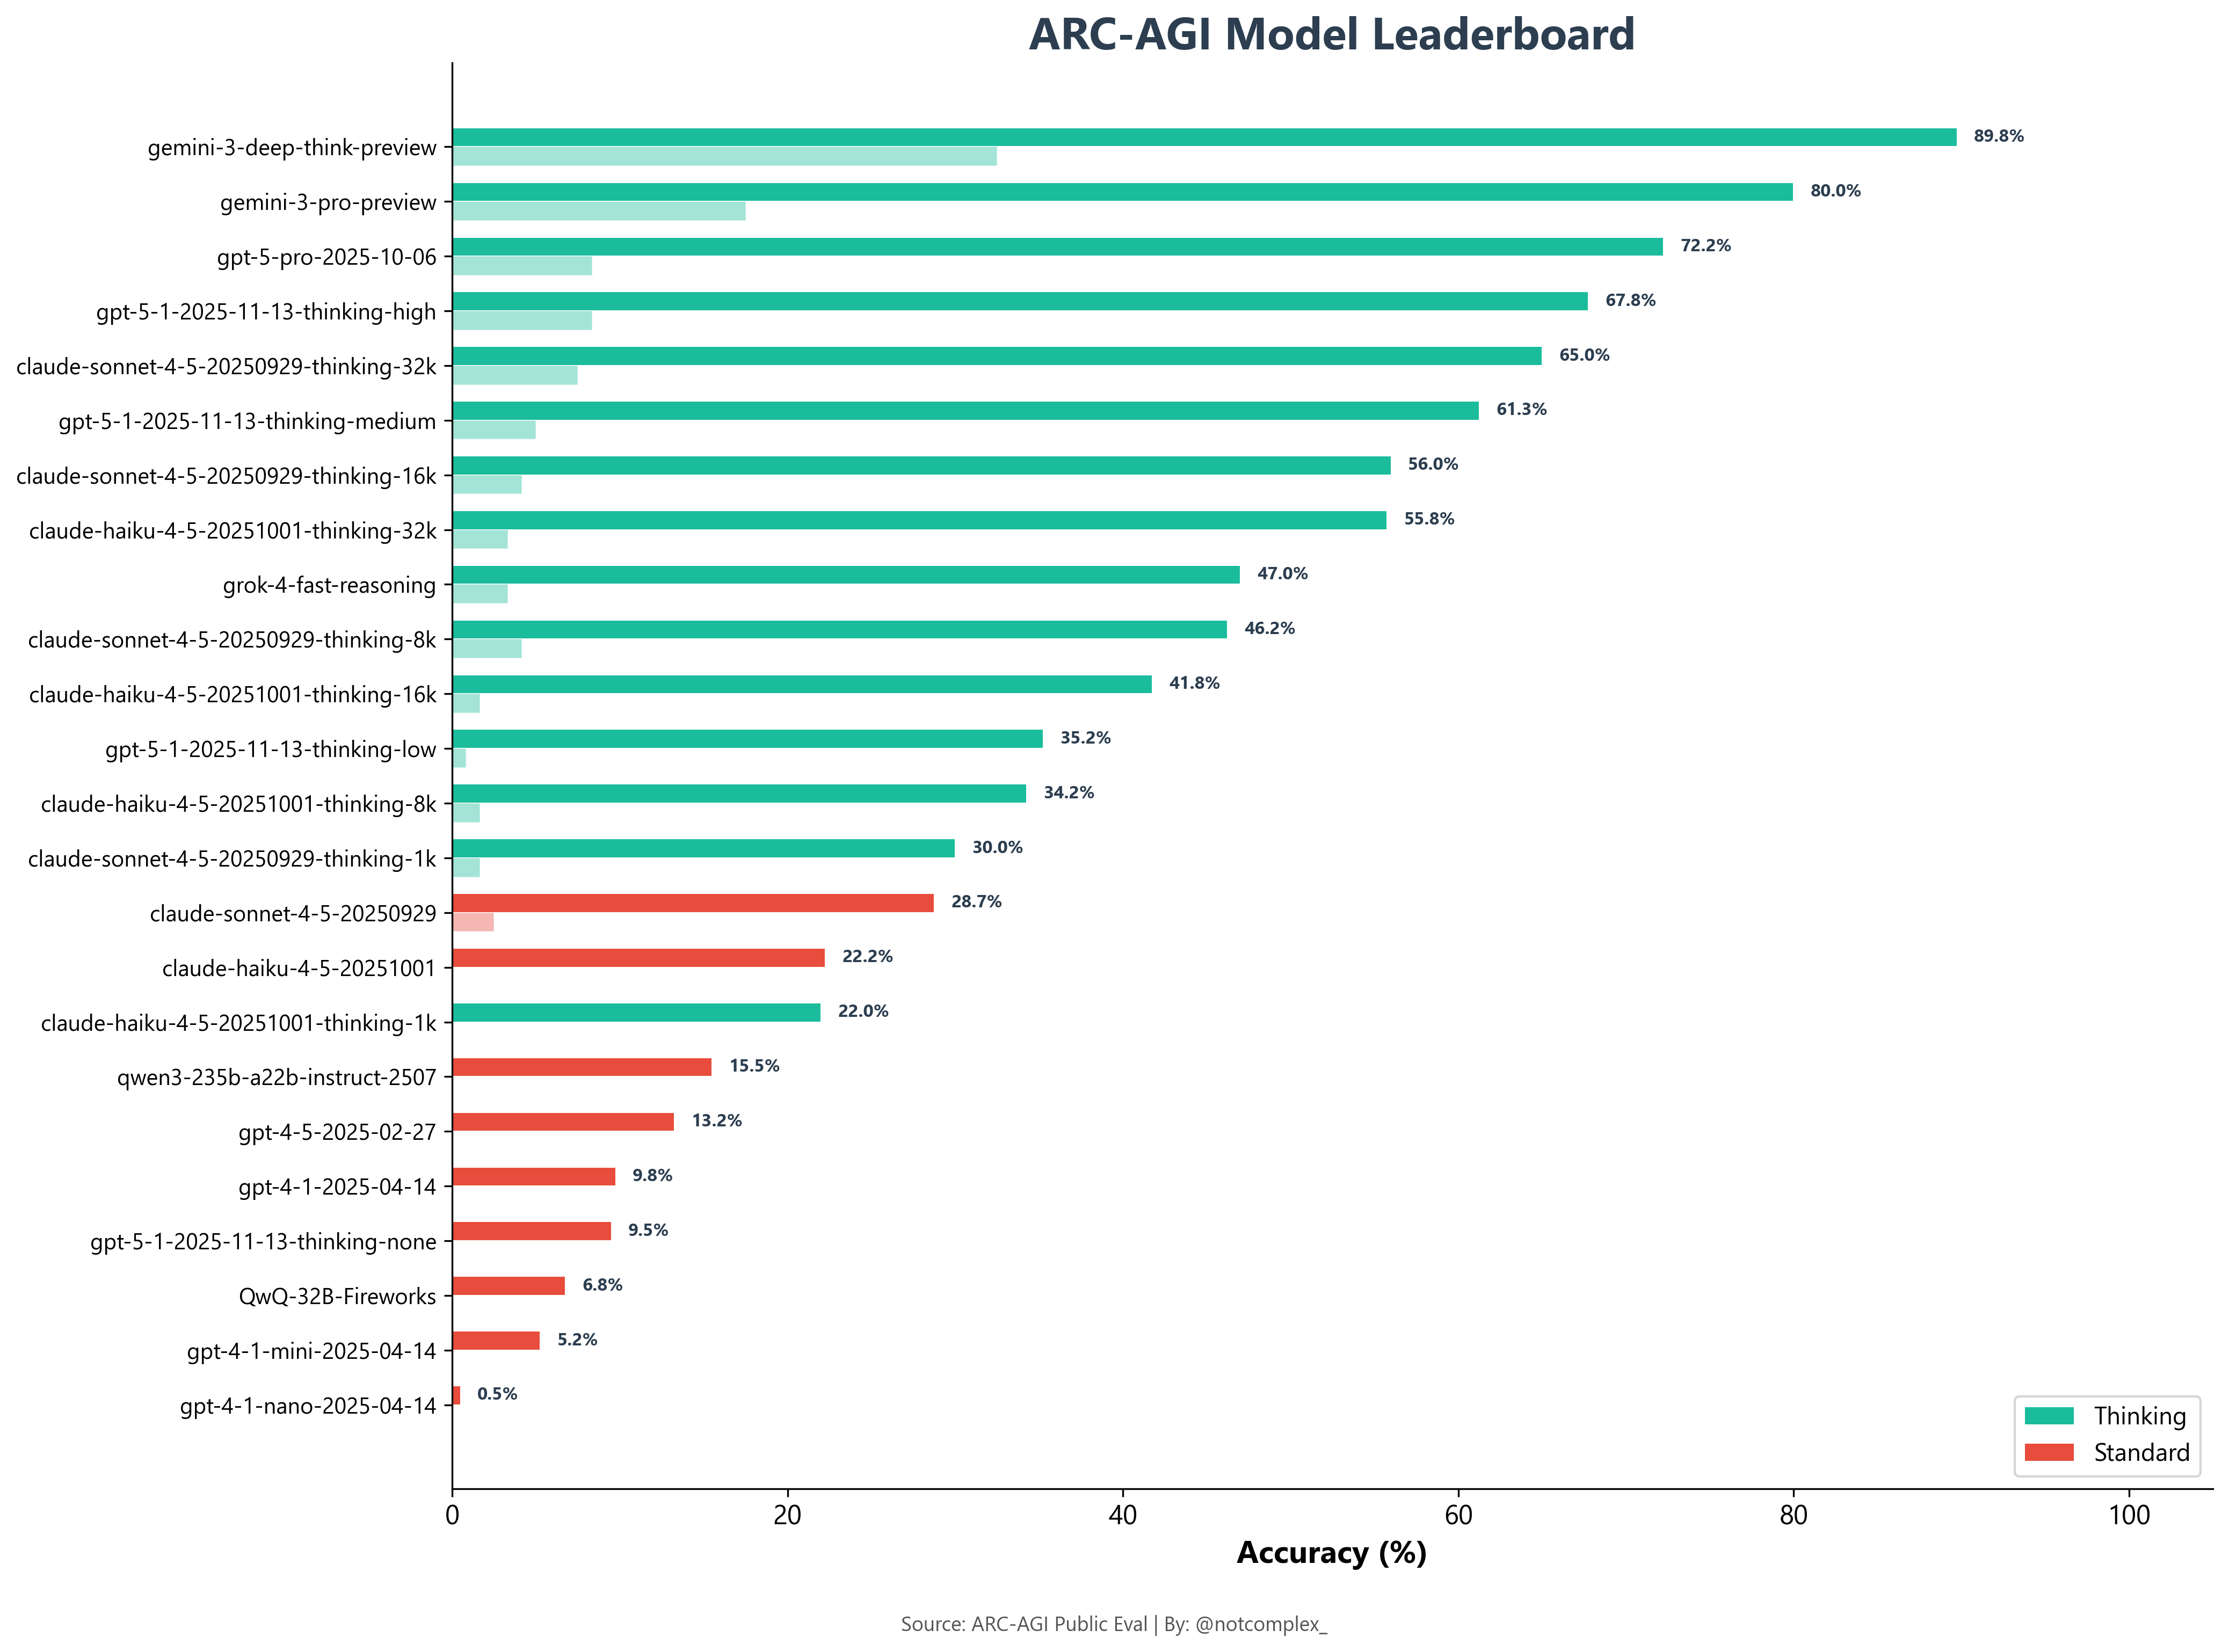
\includegraphics[width=\textwidth]{figures/fig1_leaderboard.png}
    \caption{ARC-AGI model leaderboard showing accuracy on V1 (solid bars) and V2 (faded bars). Teal indicates Thinking models; coral indicates Standard models.}
    \label{fig:leaderboard}
\end{figure}

% --- 3.2 The Response Matrix ---
\subsection{The Response Matrix: Guttman Structure}
\label{sec:guttman}

When models are sorted by total accuracy (best $\rightarrow$ worst) and tasks are sorted by pass rate (easy $\rightarrow$ hard), the response matrix reveals a striking staircase pattern characteristic of a Guttman scale (Figure~\ref{fig:matrix}).

\begin{figure}[H]
    \centering
    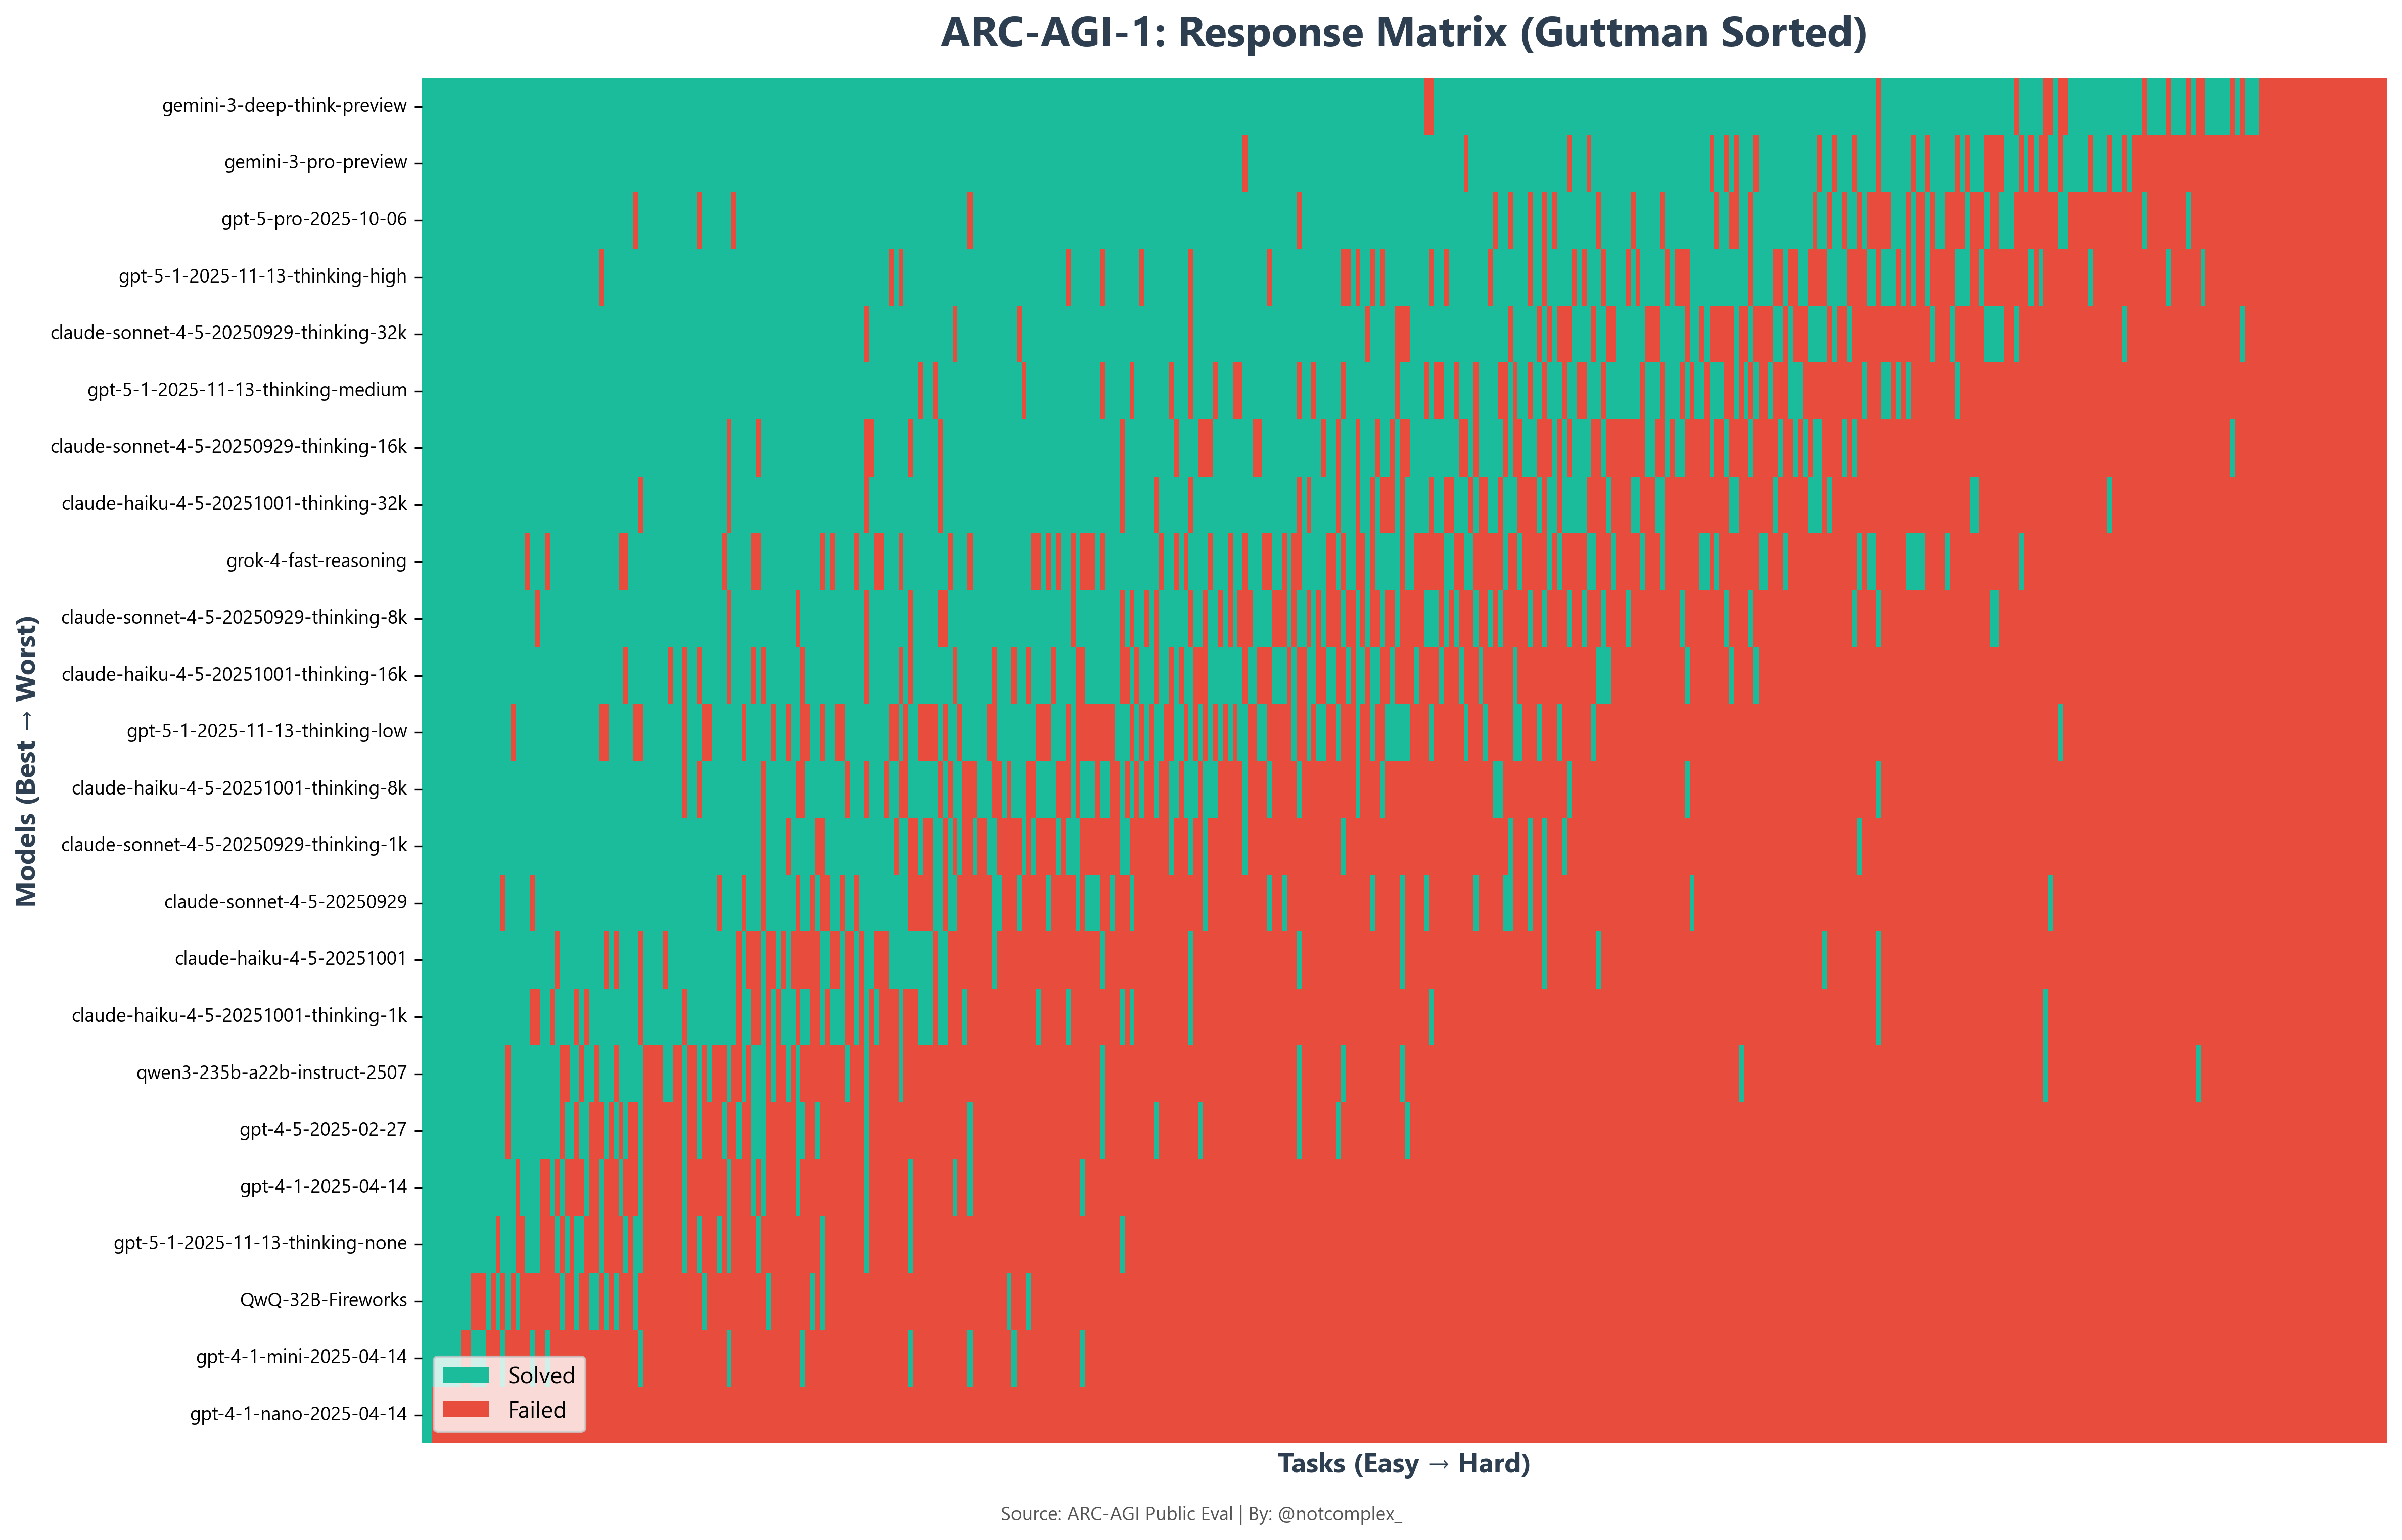
\includegraphics[width=\textwidth]{figures/fig2_response_matrix_v1.png}
    \caption{ARC-AGI-1 response matrix, Guttman-sorted. The staircase pattern indicates that tasks form a cumulative difficulty scale: models that solve harder tasks also solve all easier ones. Isolated green cells in the red region represent ``lucky wins''---anomalous correct responses on otherwise-too-hard tasks.}
    \label{fig:matrix}
\end{figure}

This visual pattern is confirmed quantitatively: Loevinger's $H = 0.779$, well above the $H > 0.5$ threshold for a ``strong'' scale. This means ARC-AGI behaves like a ruler---models are arrayed along a single difficulty continuum, and ``solving harder tasks implies solving easier ones'' holds with high fidelity.

% --- 3.3 Dimensionality ---
\subsection{Dimensionality: One Factor Rules All}
\label{sec:dimensionality}

Principal component analysis of the 25 $\times$ 372 response matrix reveals a dominant first component (Figure~\ref{fig:scree}):

\begin{itemize}
    \item \textbf{PC1:} 48.7\% of variance
    \item \textbf{PC2:} 8.8\% of variance
    \item \textbf{PC1+PC2:} 57.4\% cumulative
\end{itemize}

The large gap between PC1 and PC2 (a 5.5:1 ratio) strongly suggests \textit{essential unidimensionality}---ARC-AGI measures one dominant latent factor, analogous to the ``$g$-factor'' in human psychometrics.

\begin{figure}[H]
    \centering
    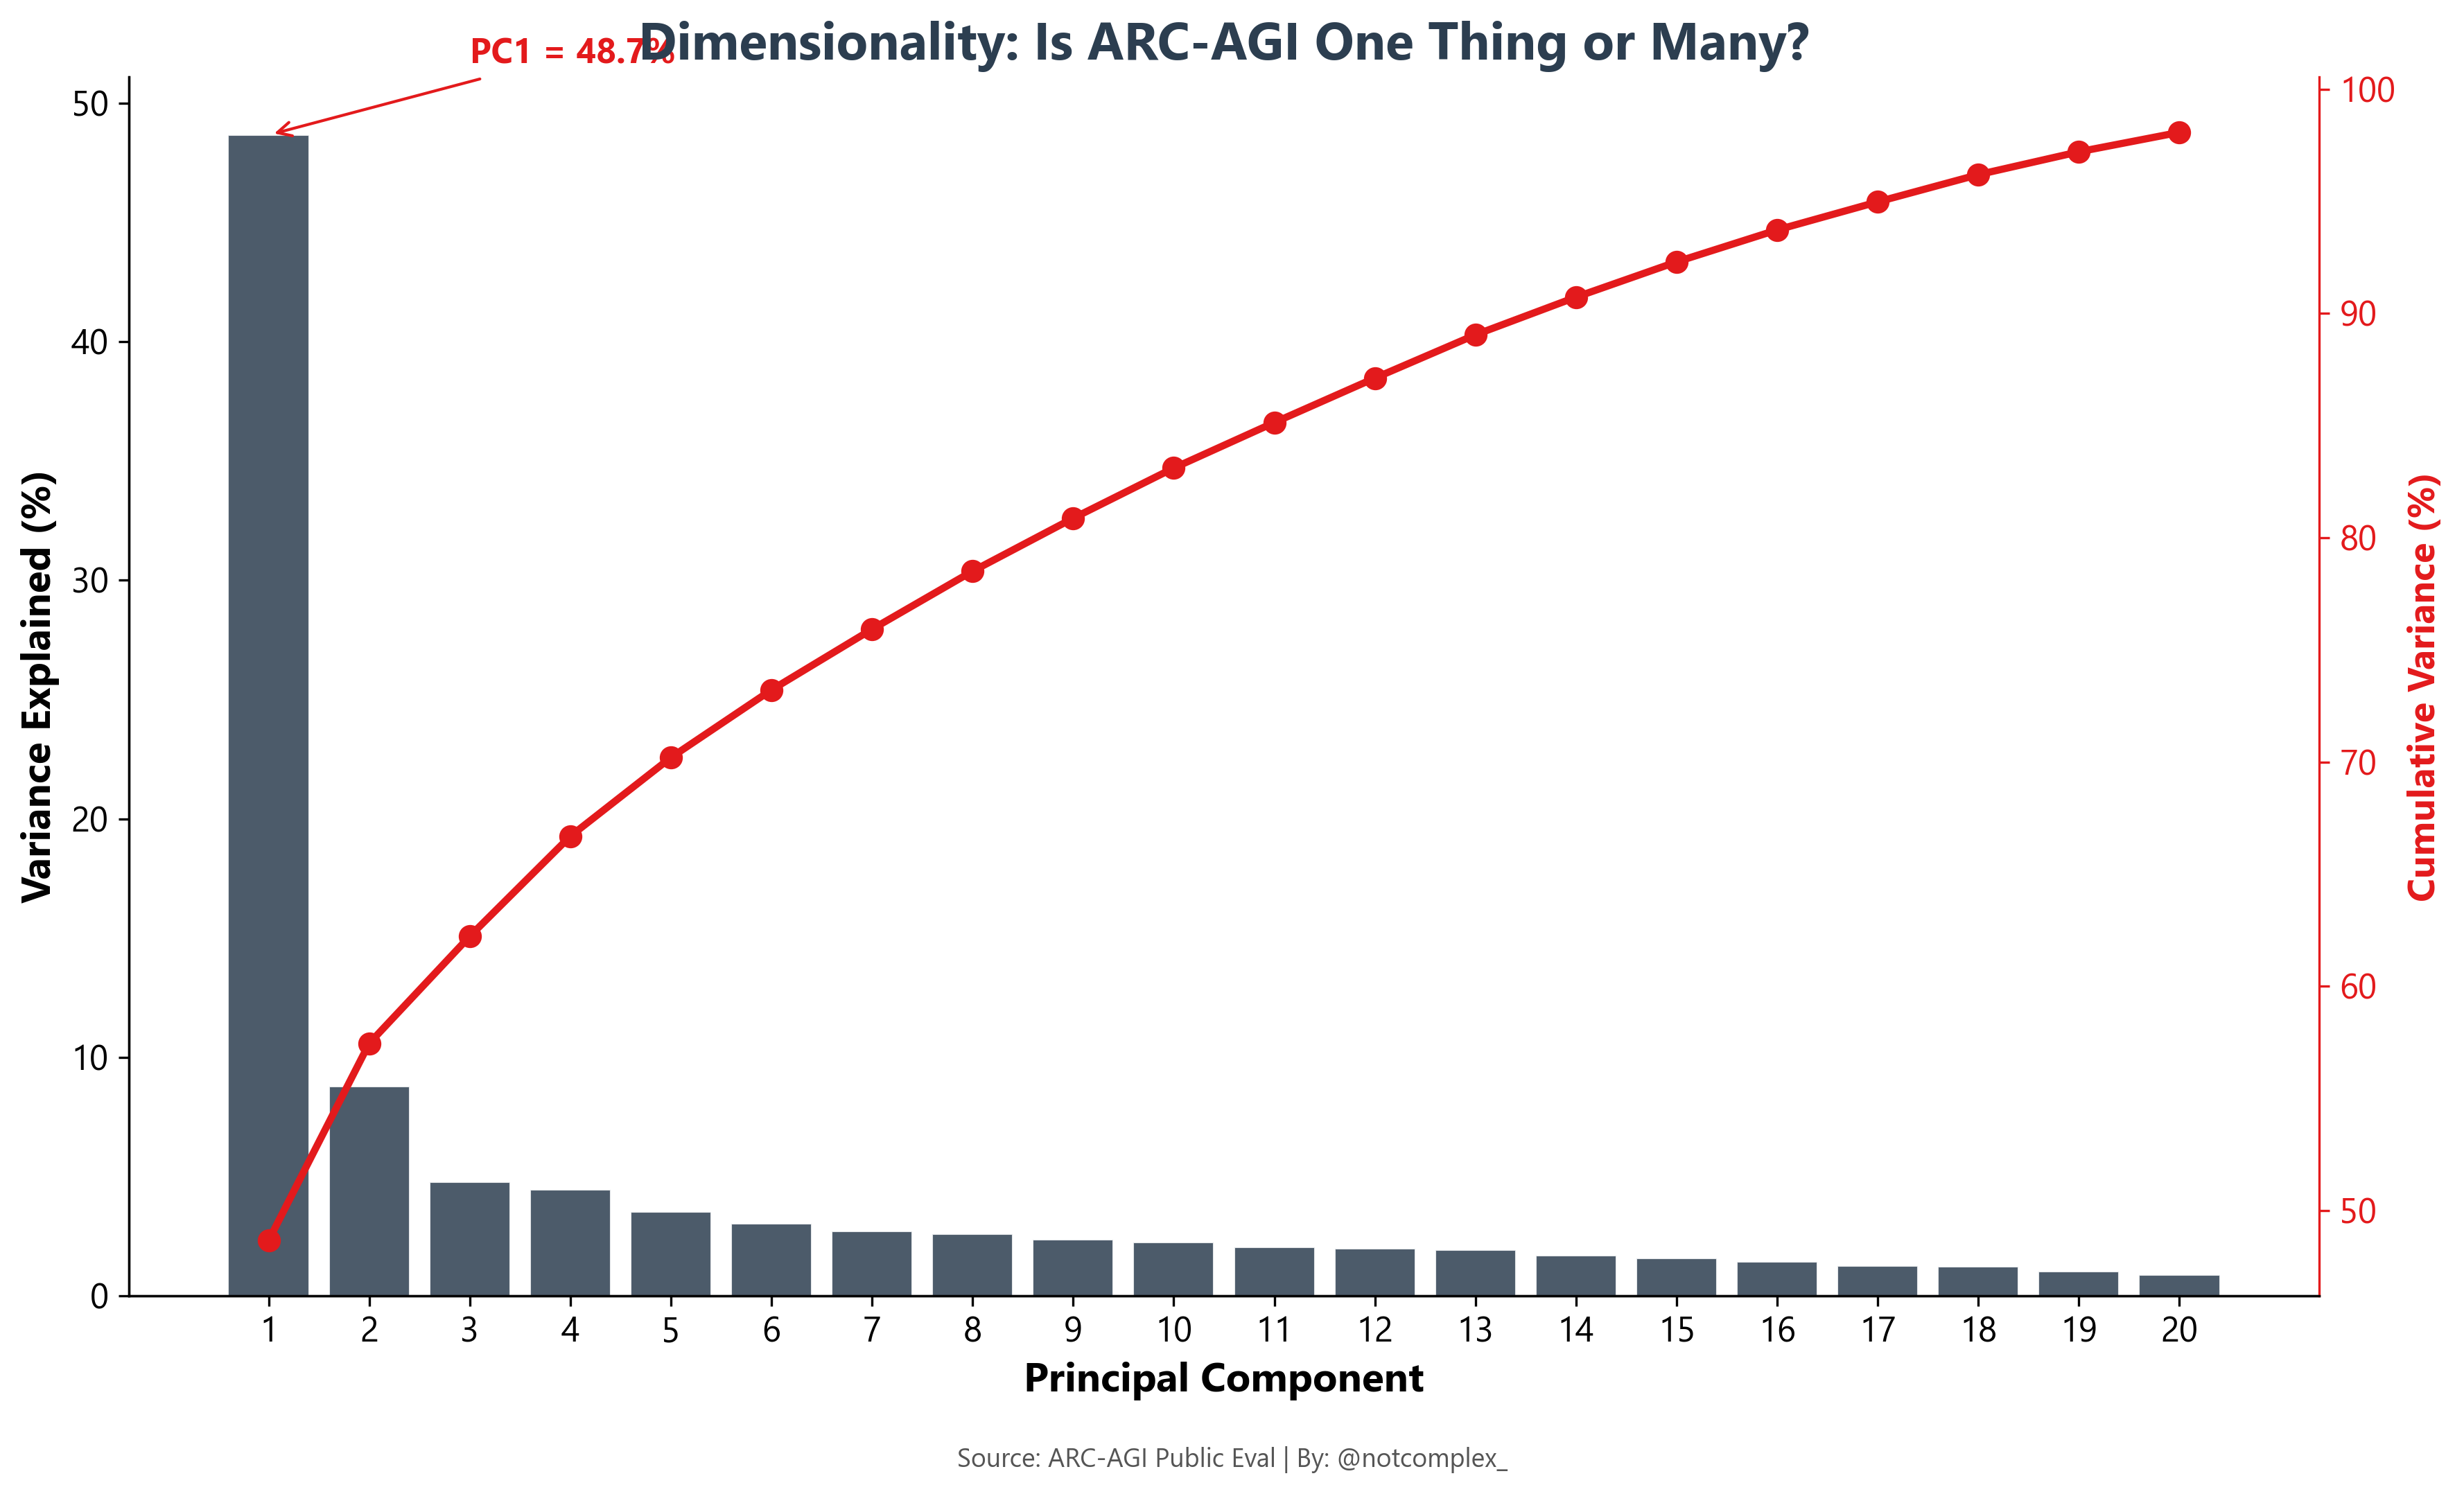
\includegraphics[width=0.9\textwidth]{figures/fig3_scree_plot.png}
    \caption{PCA scree plot. PC1 alone captures 48.7\% of variance, with a sharp ``elbow'' at PC2. The red line shows cumulative variance.}
    \label{fig:scree}
\end{figure}

% --- 3.4 The Determinism Problem ---
\subsection{The Determinism Problem}
\label{sec:determinism}

A core methodological insight of this analysis: \textbf{LLMs are deterministic test-takers}. Unlike human examinees, who produce stochastic responses (influenced by attention, guessing, fatigue), an LLM with a fixed API configuration will produce the same answer to the same task every time.

This determinism breaks classical Rasch diagnostics. The Outfit Mean-Square statistic, which measures the deviation of a person's response pattern from the Rasch model's prediction, relies on comparing observed residuals to expected variance. When the ``person'' is deterministic, the residual structure collapses: every model's response pattern is \textit{perfectly} consistent with itself, producing Outfit MSQ values that are uninterpretable under the standard null model (random guessing with given ability).

The observed symptom: traditional $p$-values are uniformly 1.000 for every model---a diagnostic anomaly that initially appeared to suggest a bug in the analysis pipeline but in fact reflects a fundamental incompatibility between classical psychometric assumptions and deterministic test-takers.

\textbf{Our solution:} We implement a permutation-based inference framework using a swap algorithm with 200 iterations. The shuffle preserves row marginals (model total scores) and column marginals (task pass rates) while randomizing the internal association structure. This generates null distributions for Outfit MSQ and Loevinger's $H$ under the null hypothesis of ``no structure beyond what marginal totals imply.''

The results (Table~\ref{tab:scale_metrics}) confirm that the observed $H = 0.779$ represents genuine scale structure, not merely an artifact of skewed marginals.

\begin{table}[H]
\centering
\caption{Global scale metrics from permutation-based inference.}
\label{tab:scale_metrics}
\begin{tabular}{lr}
\toprule
\textbf{Metric} & \textbf{Value} \\
\midrule
Loevinger's $H$ & 0.779 \\
$N$ Models & 24 \\
$N$ Tasks (with variance) & 372 \\
Permutation iterations & 200 \\
\bottomrule
\end{tabular}
\end{table}

% --- 3.5 The Cognitive Map ---
\subsection{The Cognitive Map}
\label{sec:cognitive_map}

Projecting model performance onto the first two principal components creates a ``cognitive map'' (Figure~\ref{fig:cogmap}). PC1 separates models by overall ability (left = weak, right = strong). PC2, which explains only 8.8\% of variance, captures minor secondary variation.

\begin{figure}[H]
    \centering
    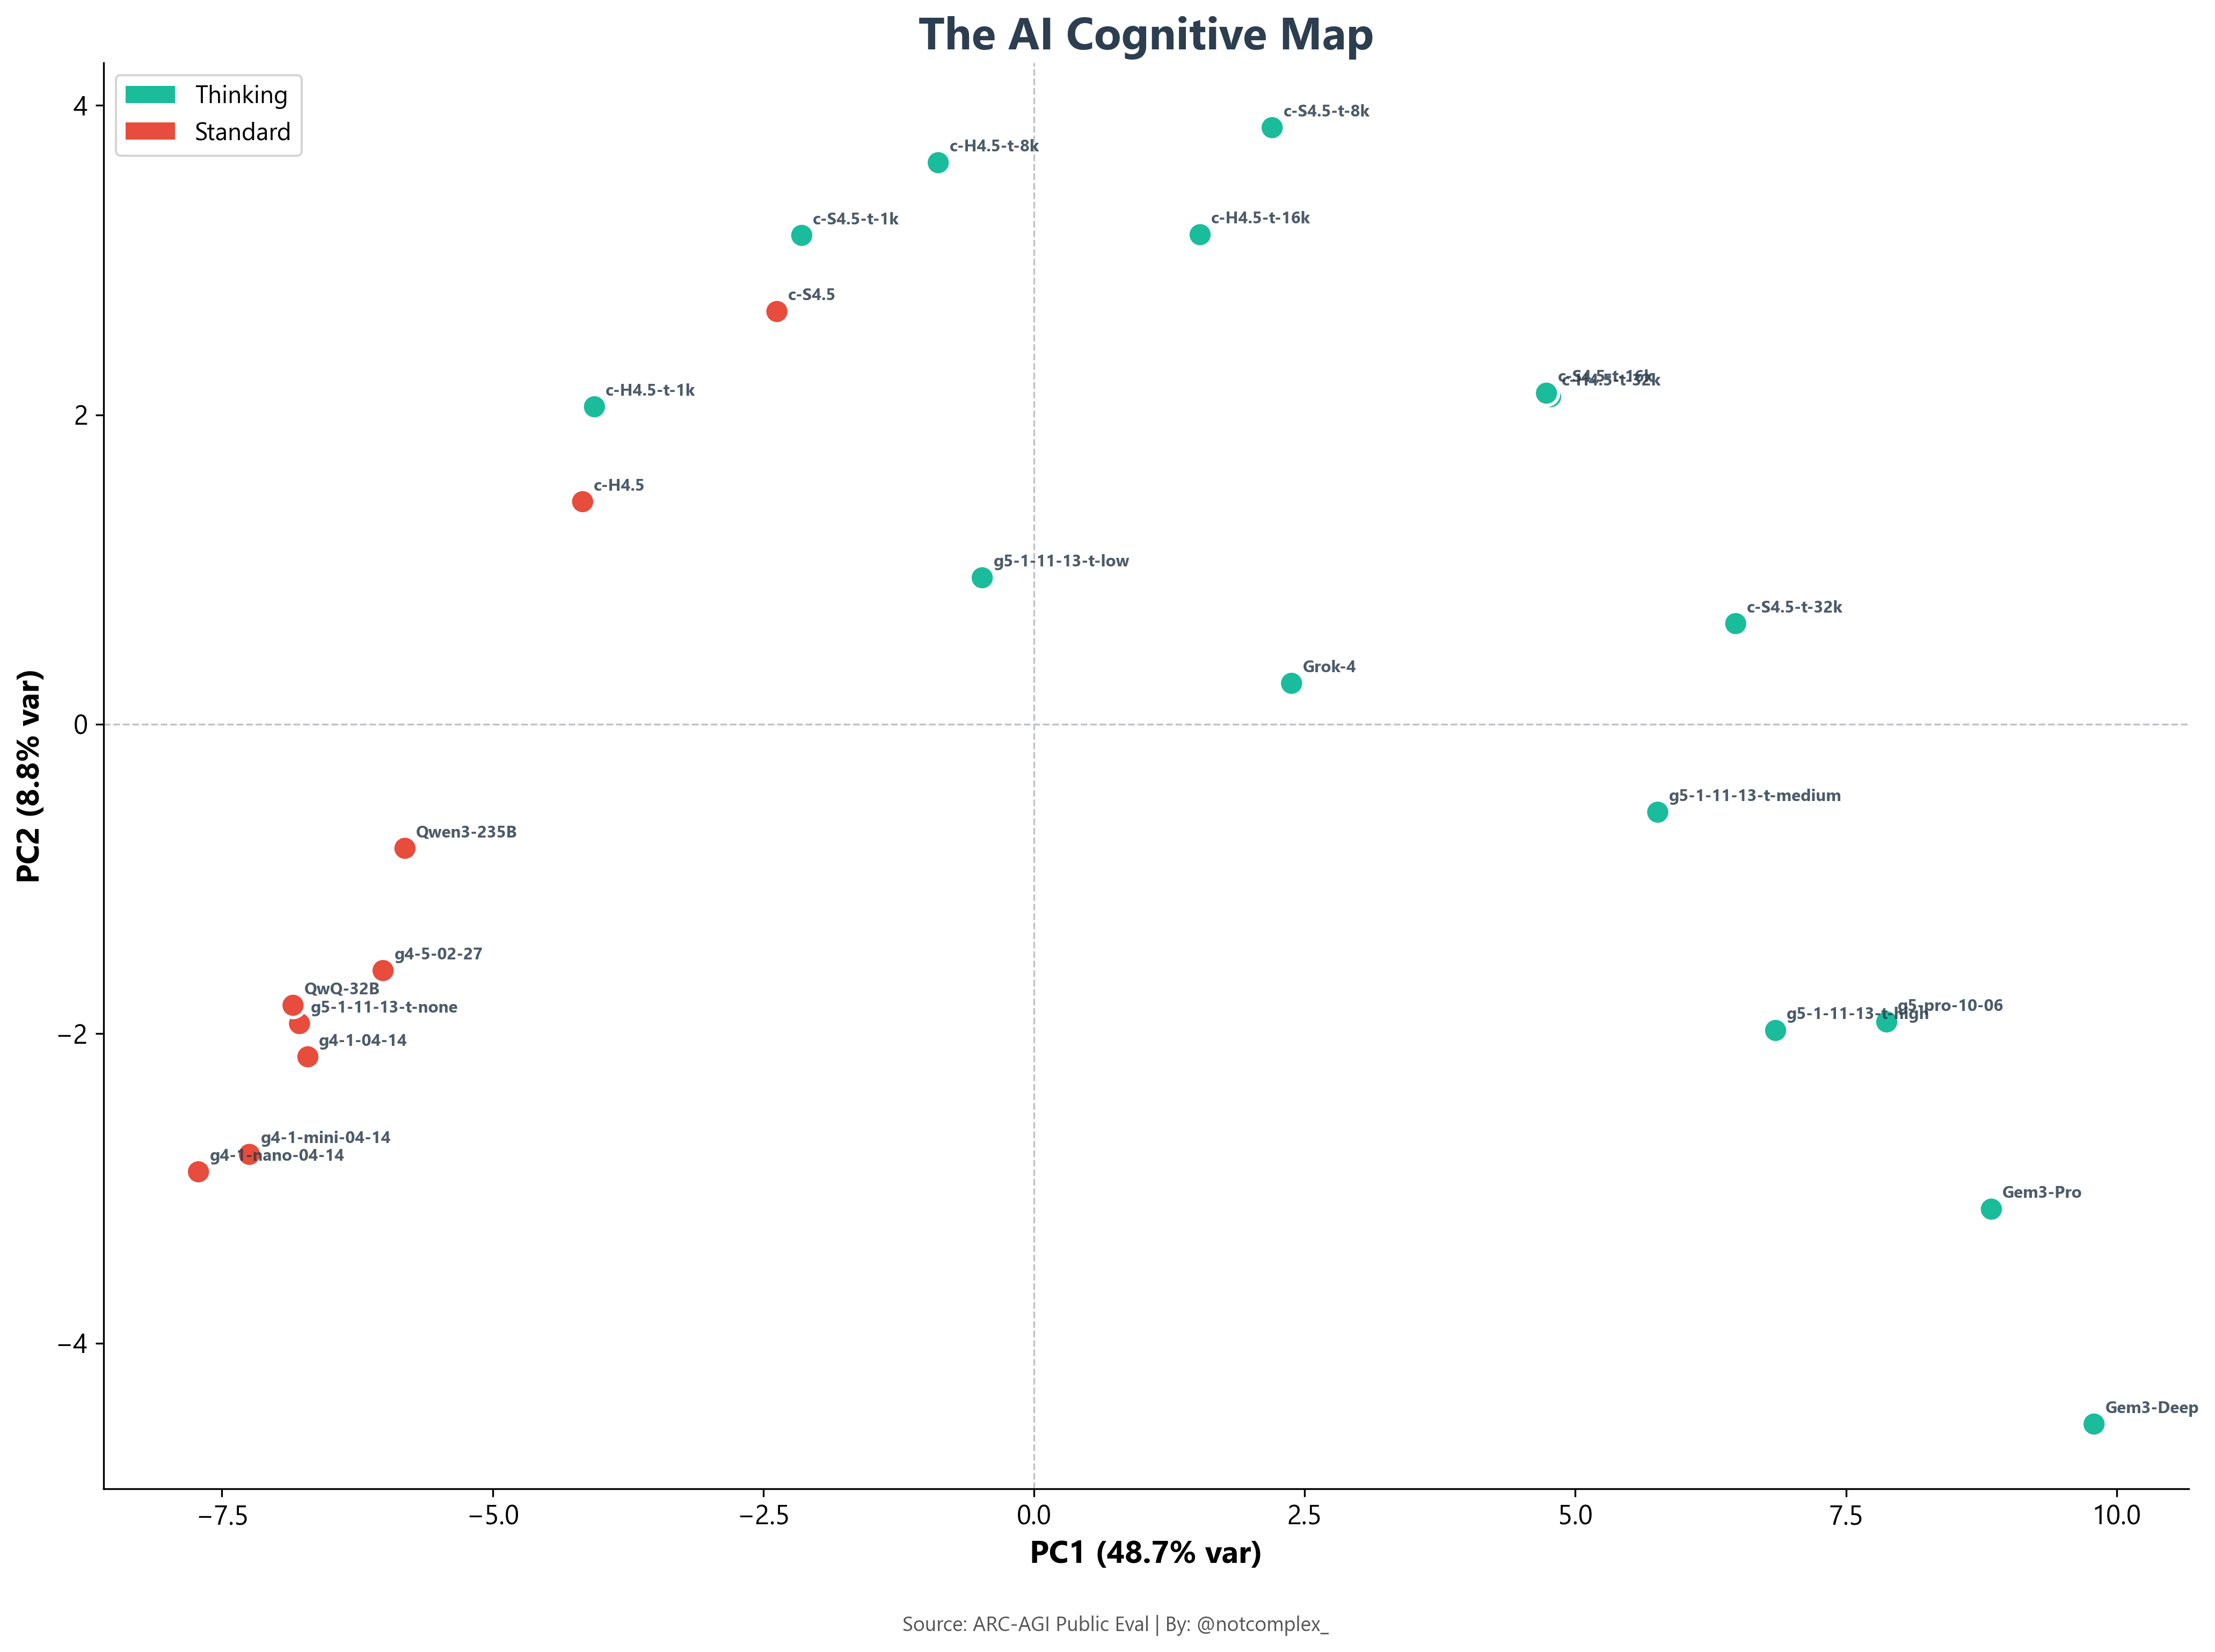
\includegraphics[width=0.9\textwidth]{figures/fig4_cognitive_map.png}
    \caption{PCA cognitive map. Each point is a model; position reflects performance similarity. Thinking models (teal) occupy the right (higher ability) region of PC1.}
    \label{fig:cogmap}
\end{figure}

Critically, Thinking and Standard models are \textit{not separated along PC2}---they differ only in their PC1 score. This supports the interpretation that extended inference does not unlock qualitatively different reasoning; it increases computational depth along the same dimension.

% --- 3.6 Ability Estimates ---
\subsection{Rasch Ability Estimates and AI-IQ Scores}
\label{sec:iq}

Using the logit-transformed accuracy as a Rasch ability proxy ($\theta = \log \frac{p}{1-p}$), we derive latent ability estimates and scale them to an IQ-like metric (mean = 100, SD = 15). The resulting ``AI-IQ'' scores (Figure~\ref{fig:ability}) reveal:

\begin{itemize}
    \item \textbf{Gemini 3 Deep-Think} leads at IQ 130 ($\theta = 3.17$), placing it more than 2 standard deviations above the mean model.
    \item \textbf{All Standard models} fall below IQ 100, with GPT-4.1-nano at the floor (IQ 52, $\theta = -6.91$).
    \item The gap between the highest Thinking model (Gemini, IQ 130) and the highest Standard model (Claude Sonnet 4.5 base, IQ 99) is approximately 2 SD---a dramatic effect size.
\end{itemize}

\begin{figure}[H]
    \centering
    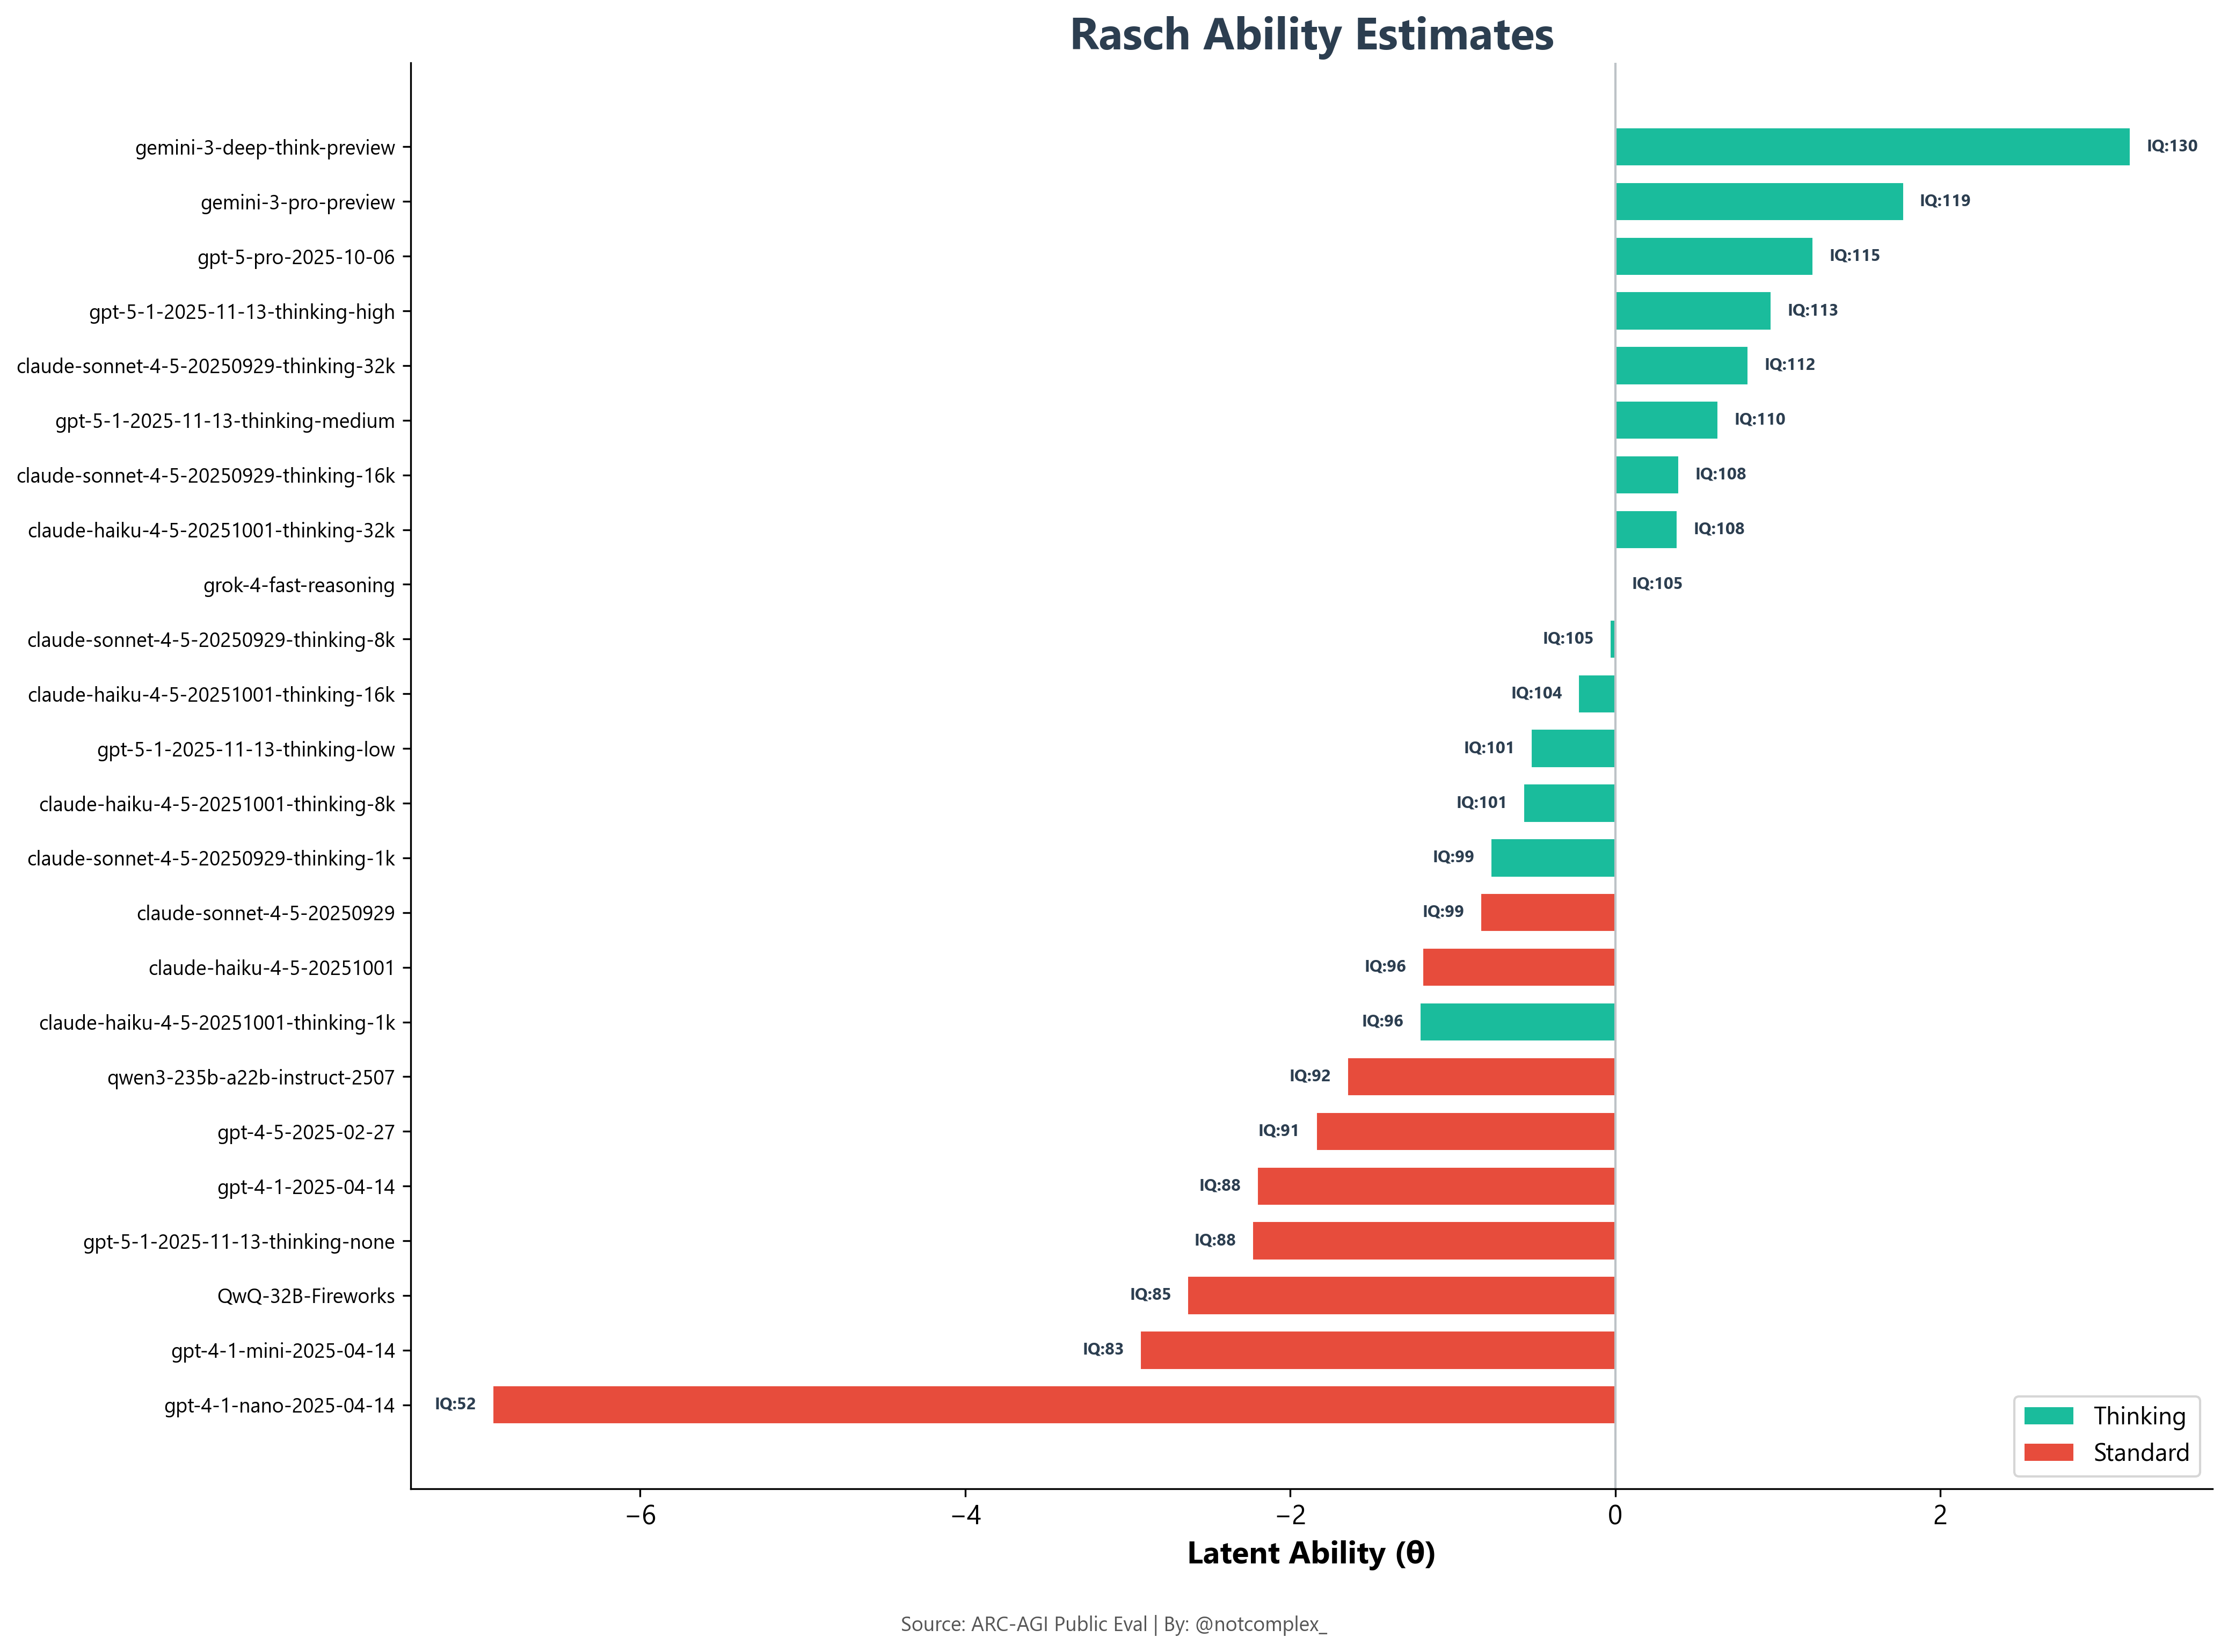
\includegraphics[width=\textwidth]{figures/fig5_ability.png}
    \caption{Rasch ability estimates ($\theta$) with AI-IQ scaling. The zero line represents the median model. Teal = Thinking; coral = Standard.}
    \label{fig:ability}
\end{figure}

% --- 3.7 Model Taxonomy ---
\subsection{Model Taxonomy: The Family Tree}
\label{sec:taxonomy}

Hierarchical cluster analysis (Ward's method, Jaccard distance) reveals the genealogical structure of model performance (Figure~\ref{fig:dendrogram}). Models cluster primarily by vendor and reasoning configuration:

\begin{itemize}
    \item The \textbf{OpenAI GPT-5.1 thinking variants} form a tight cluster, differing mainly in the thinking-token budget allocated.
    \item \textbf{Claude Haiku} and \textbf{Claude Sonnet} models with similar thinking budgets cluster together, suggesting that model size matters less than thinking allocation for ARC-AGI.
    \item \textbf{GPT-4.1-nano} is a clear outlier, joining the tree only at maximum distance (zero tasks solved).
\end{itemize}

\begin{figure}[H]
    \centering
    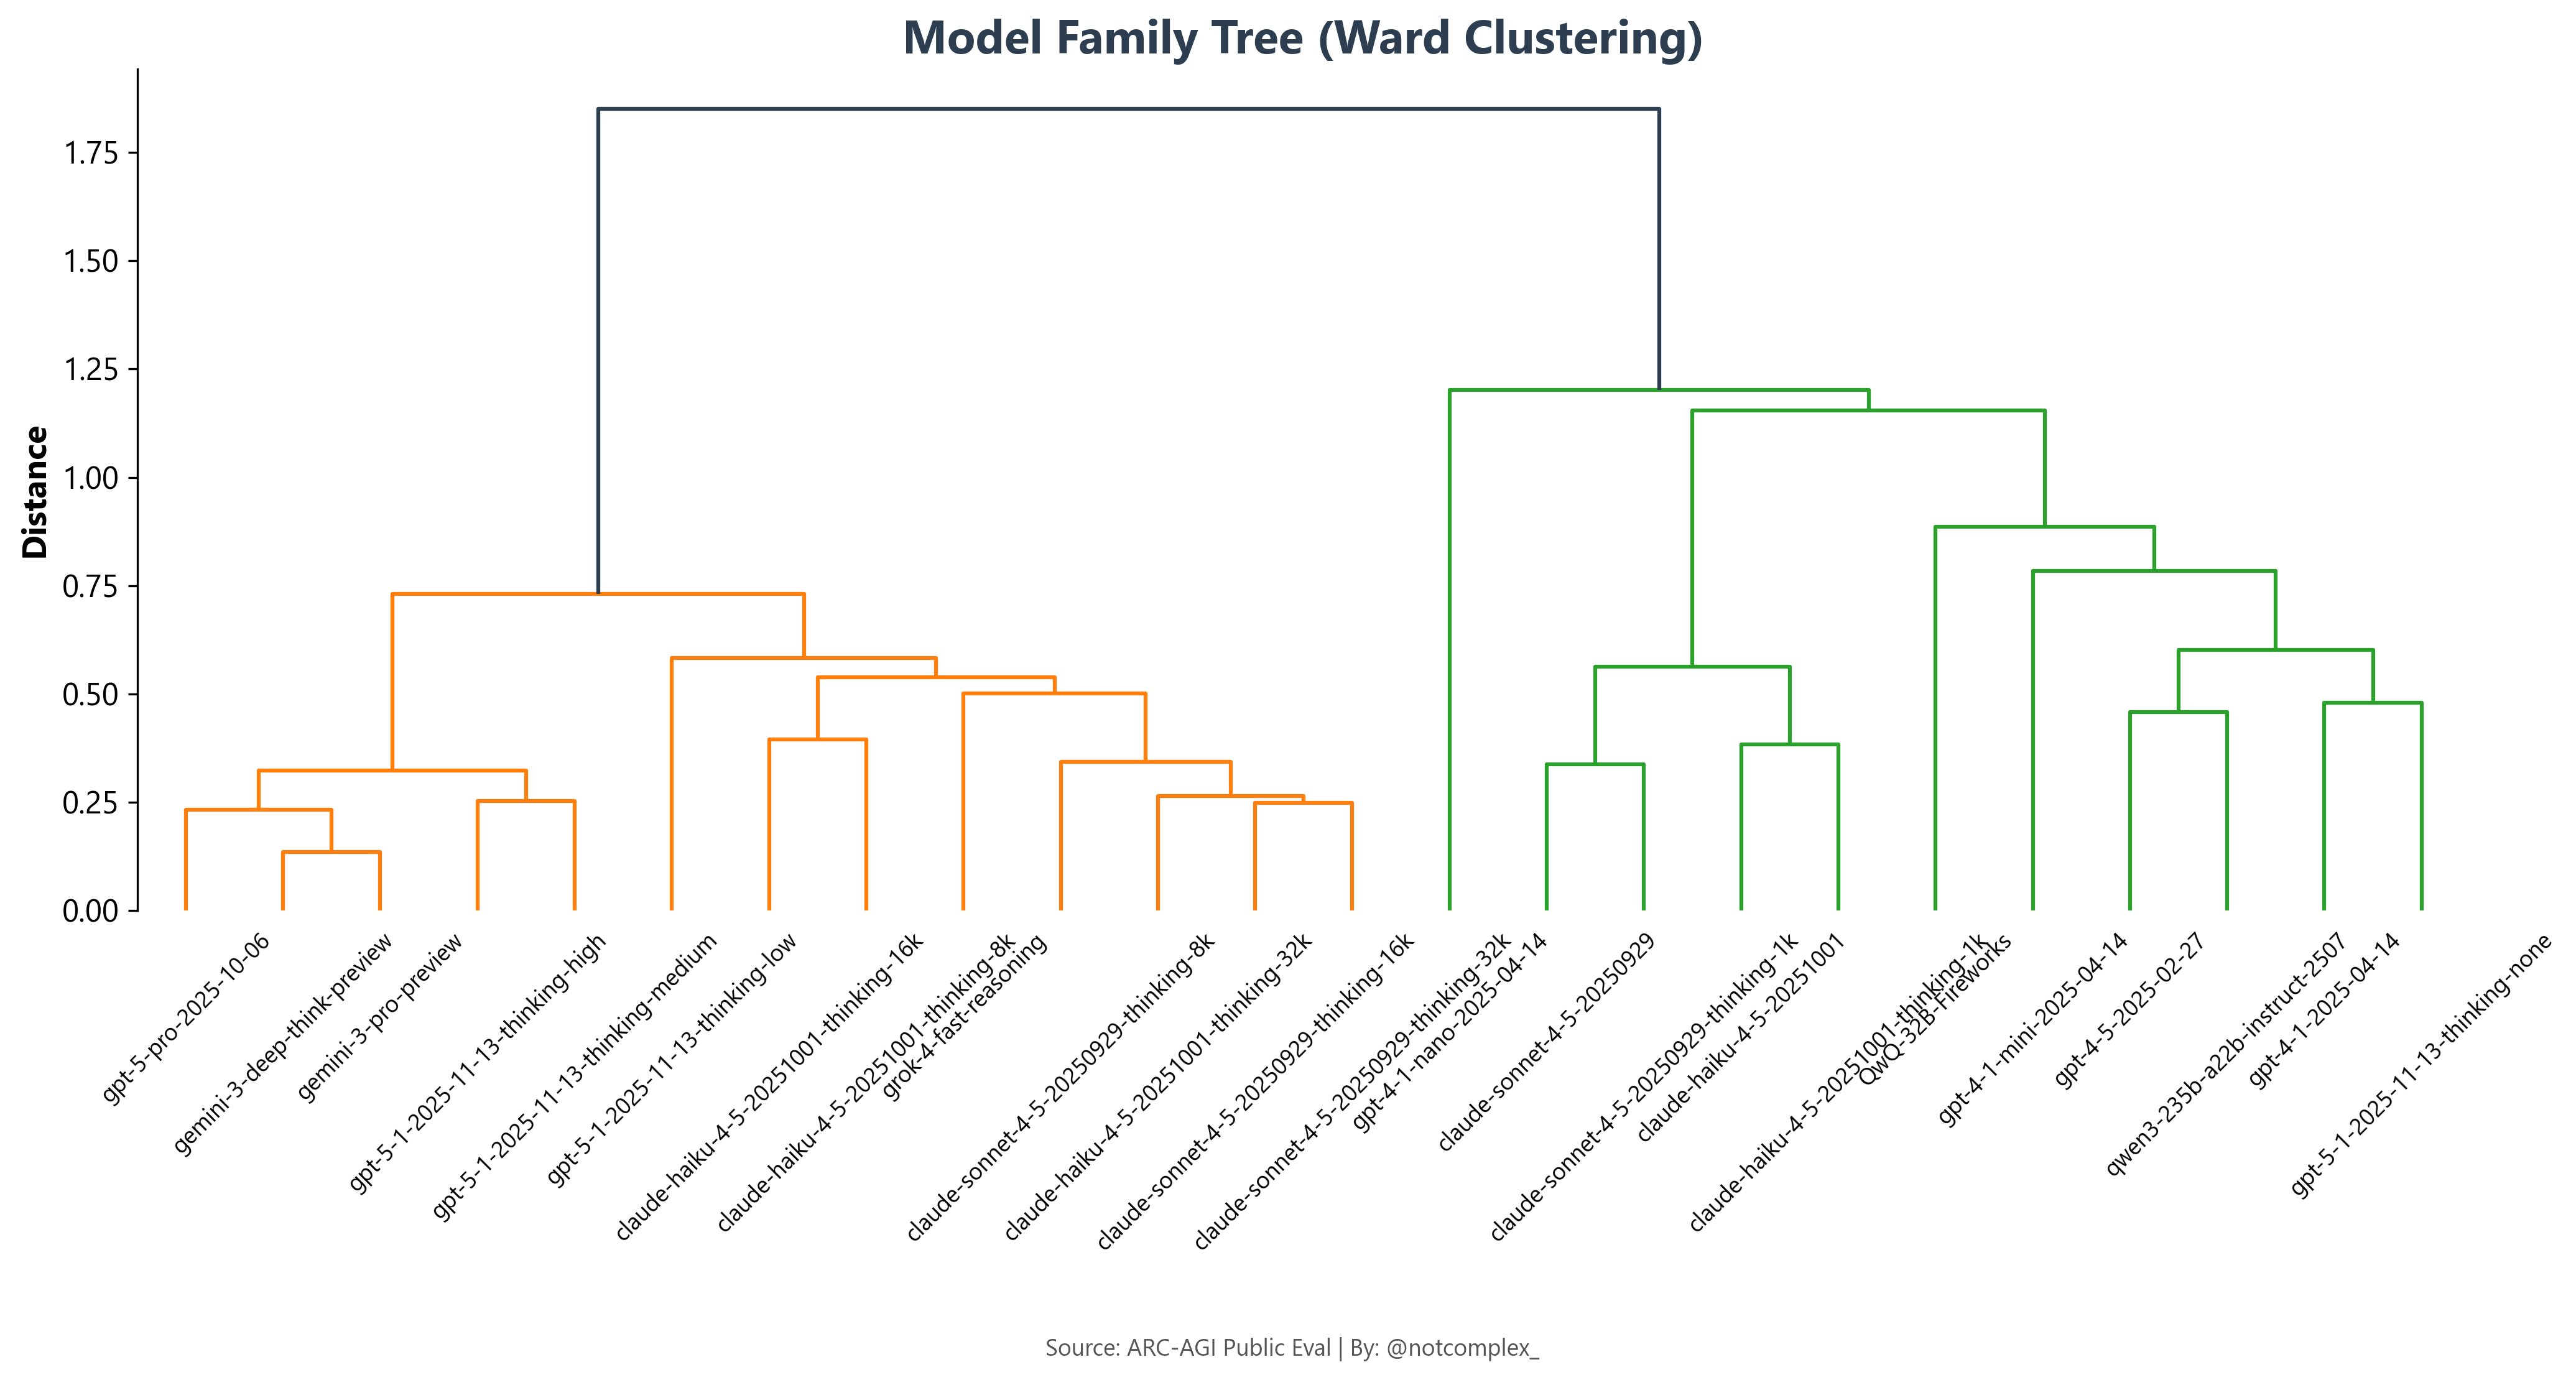
\includegraphics[width=\textwidth]{figures/fig6_dendrogram.png}
    \caption{Model family tree (Ward linkage on Jaccard distance). Models with similar response patterns are grouped together, revealing ``reasoning families'' that transcend vendor boundaries.}
    \label{fig:dendrogram}
\end{figure}

% --- 3.8 Task Difficulty ---
\subsection{Task Difficulty Distribution}
\label{sec:difficulty}

The distribution of task difficulty (Figure~\ref{fig:difficulty}) shows that ARC-AGI-1 evaluates a broad range of difficulty levels, with a roughly bimodal structure: a cluster of ``easy'' tasks solved by most models and a long tail of extremely difficult tasks solved by only the top performers.

\begin{figure}[H]
    \centering
    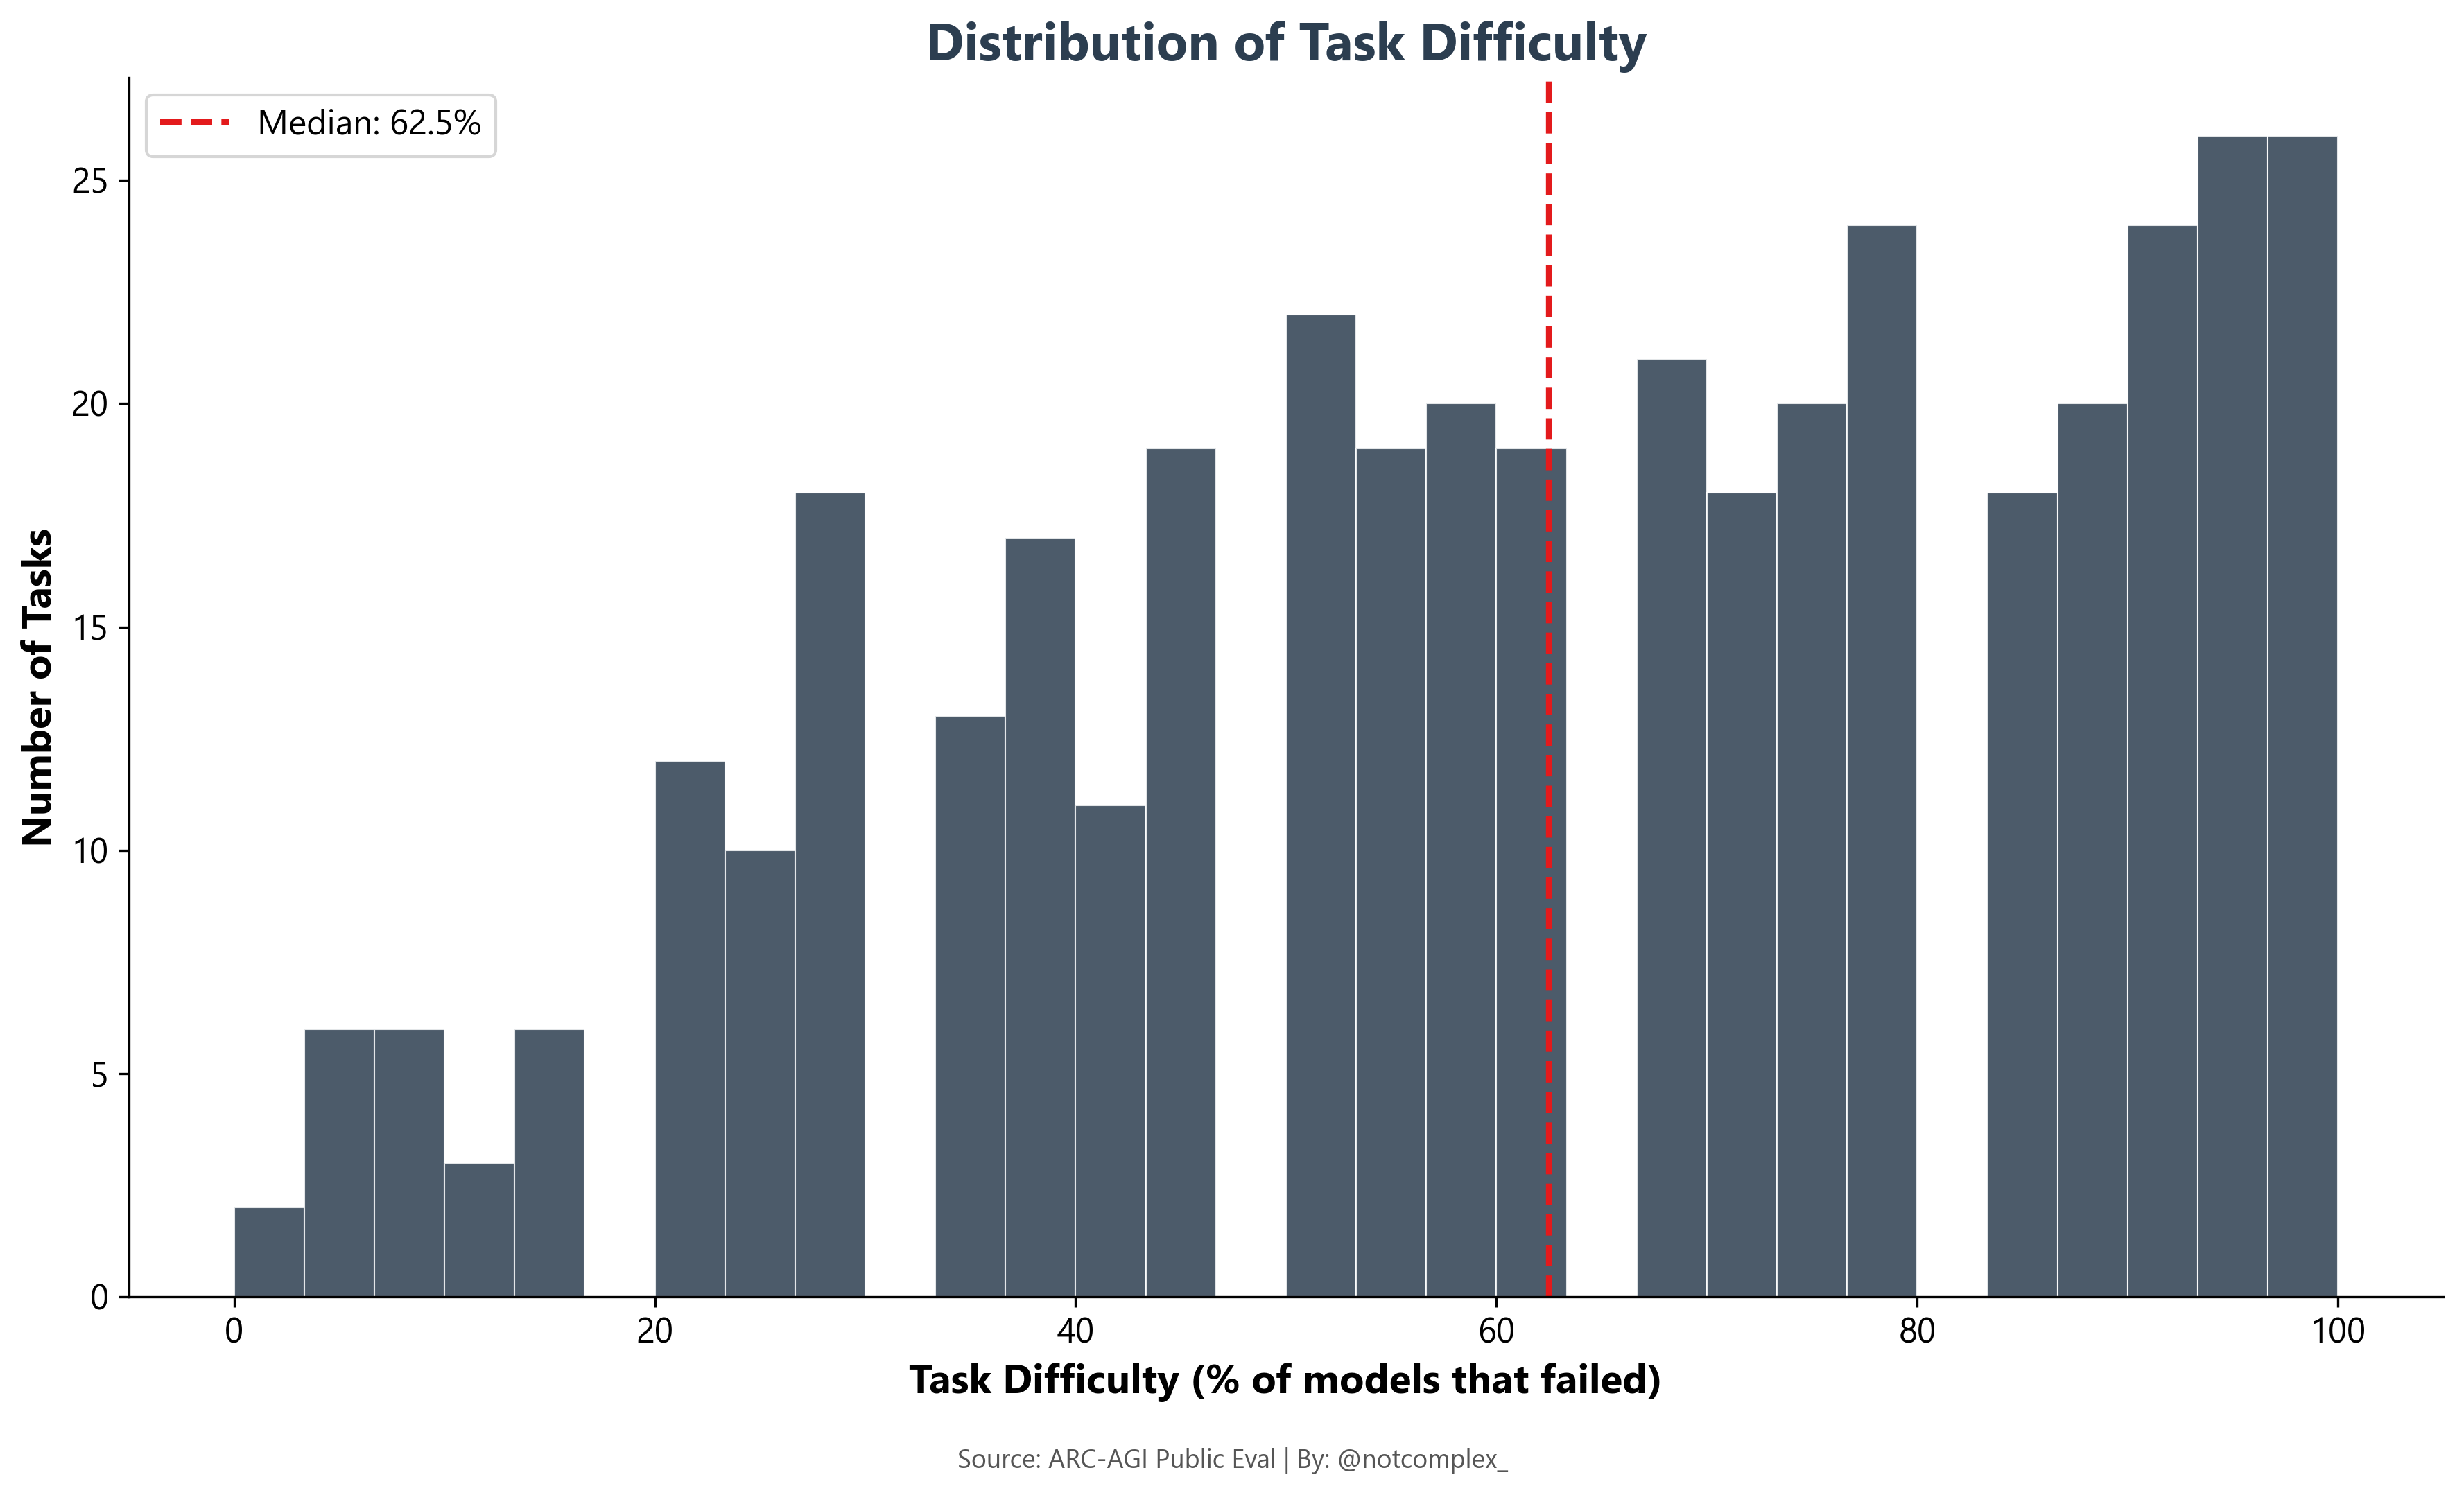
\includegraphics[width=0.9\textwidth]{figures/fig7_difficulty_dist.png}
    \caption{Distribution of task difficulty (percentage of models failing each task). Higher values = harder tasks.}
    \label{fig:difficulty}
\end{figure}

% =============================================================================
\section{Discussion}
\label{sec:discussion}

\subsection{ARC-AGI Measures One Thing}

The convergent evidence from PCA (48.7\% on PC1, 5.5:1 ratio vs.\ PC2), Loevinger's $H$ (0.779), and the visual Guttman staircase all point to the same conclusion: \textbf{ARC-AGI is essentially unidimensional}. It measures a single latent factor that we might call ``abstract reasoning ability'' or, more precisely, ``the capacity to infer visual transformation rules from few examples.''

This is both a strength and a limitation. As a strength, unidimensionality means ARC-AGI scores are interpretable---a higher score genuinely means ``better at this kind of reasoning,'' not ``better at a different subset of tasks.'' As a limitation, it means ARC-AGI cannot distinguish between \textit{types} of intelligence; a model that excels at spatial rotation but fails at counting will be ranked the same as one with the opposite profile.

\subsection{LLMs Are Deterministic Test-Takers}

Our most methodologically novel contribution is the identification and resolution of the ``determinism problem.'' When LLMs are evaluated at fixed settings (temperature = 0, no sampling), they behave like a lookup table: the same input always produces the same output. This violates the stochastic assumptions embedded in virtually all classical psychometric models, which assume that test performance contains a random error component.

The practical consequence is that traditional Rasch diagnostics (Outfit MSQ, Zh statistics) produce degenerate results---$p$-values of 1.000 for every model. This does not mean the Rasch model is wrong; it means the \textit{inference machinery} is wrong. Our permutation-based fix preserves the Rasch framework while replacing the parametric null model with an empirical one derived from the data itself.

This issue will apply to \textit{any} psychometric analysis of AI systems administered under deterministic conditions. It represents a systematic blind spot in the emerging field of ``AI psychometrics'' that has not, to our knowledge, been previously documented.

\subsection{Thinking $\neq$ Different, Just Better}

The cognitive map (Figure~\ref{fig:cogmap}) and ability estimates (Figure~\ref{fig:ability}) tell a clear story: Thinking models (extended inference with chain-of-thought) and Standard models occupy the \textit{same latent space}. They are separated along PC1 (ability) but not along PC2 or higher dimensions. The implication:

\begin{quote}
    \textit{Extended thinking time buys more computation on the same reasoning scale. It does not unlock a qualitatively different form of intelligence.}
\end{quote}

This has direct relevance to the ``scaling $\rightarrow$ AGI'' debate. If thinking tokens simply shift a model rightward on a unidimensional scale, then the path from current models to human-level abstract reasoning is one of degree, not kind---and we should expect diminishing returns as models approach the ceiling of what this single dimension can capture.

\subsection{V2 as a Harder Ruler}

ARC-AGI-2 compresses the performance range dramatically (maximum 32.5\% vs.\ 96.0\% on V1). This confirms that V2 is a ``harder ruler'' measuring the same construct at a higher difficulty level. The top-3 ranking is preserved across versions (Gemini Deep-Think $>$ Gemini Pro $>$ GPT-5-Pro), suggesting reliable measurement at the frontier.

The floor effect on V2---with most Standard models scoring 0.0\%---suggests that V2 may be \textit{too} difficult to provide meaningful discrimination among weaker models. The Test Information Function (not shown) confirms that V2's measurement precision is concentrated at very high ability levels.

% =============================================================================
\section{Conclusion}
\label{sec:conclusion}

We have applied classical and modern psychometric methods to ARC-AGI, the most widely cited benchmark for AI abstract reasoning. Our findings are:

\begin{enumerate}
    \item \textbf{ARC-AGI is unidimensional.} It measures a single dominant factor (PC1 = 48.7\%), and its items form a strong cumulative scale ($H = 0.779$).
    \item \textbf{LLMs break classical psychometrics.} Deterministic inference produces degenerate diagnostics. Permutation-based methods are required.
    \item \textbf{Thinking models are better, not different.} Extended inference increases ability on the same scale; it does not create new dimensions of reasoning.
    \item \textbf{ARC-AGI is a valid ruler} for ranking frontier models on abstract reasoning, with V1 providing broad discrimination and V2 providing precision at the frontier.
\end{enumerate}

The central insight is sobering for AI progress claims: the 25 frontier models tested here, spanning five vendors and two years of development, differ in \textit{degree} of a single ability, not in \textit{kind}. Whether this reflects a genuine limitation of current architectures or a limitation of the benchmark itself is an open question for future work.

% =============================================================================
\section*{Data Availability}
\label{sec:data}

All evaluation data, analysis scripts, and generated figures are available in the project repository. The response matrices, permutation test results, and model scoring can be reproduced using the \texttt{generate\_all.py} script included in the \texttt{scripts/} directory.

% =============================================================================
\end{document}
